\documentclass{beamer}
\usepackage{siunitx}

\usepackage[utf8]{inputenc}
\usetheme{Dresden}
\title{INTRO TO AI/ML}
\author{AAYUSH ARORA (EE17BTECH11003) \and AAKASH DASWANI (EE17BTECH11002) }


\begin{document}

\maketitle
\begin{frame}{QUESTION IN MATRIX FORM:}
Find the equation of the tangent to the circle,
at the point
$\begin{bmatrix}
1\\
-1\\
\end{bmatrix}$
whose centre is the point of intersection of the
straight lines
\newline
\begin{itemize}
\item (2,$1$) $\textbf{x} =  3$
\item (1,$-1$) $\textbf{x} =  1$
\end{itemize}

\end{frame}
\begin{frame}{QUESTION IN 2D FORM:}
Find the equation of the tangent to the circle,
at the point (1,-1) whose centre is the point of intersection of the
straight lines
\newline
\begin{itemize}
\item $2x+y=3$
\item $x-y=1$
\end{itemize}

\end{frame}

\begin{frame}{APPROACH (USING VECTORS) :}
$A = (1,-1)$\\
$\textbf{n}_1^{T} = (2,1)$\\
$\textbf{n}_2^{T} =  (1,-1)$\\
$p_1 = 3$\\
$p_2=1$\\

Let \\
$\textbf{n}_1^{T}  \textbf{x} = p_1$\\
$\textbf{n}_2^{T}  \textbf{x} = p_2$\\
$\begin{bmatrix}
\textbf{n}_1^{T}\\
\textbf{n}_2^{T}\\
\end{bmatrix}$
$\textbf{x} = p $\\
$\textbf{N} = (\textbf{n}_1,\textbf{n}_2)$\\
$\textbf{x} = (\textbf{N}^{T})^{-1} p $\\
$\textbf{x} = (\textbf{N}^{-T}) p$
\end{frame}

\begin{frame}
$C = 
\begin{bmatrix}
1/3,1/3\\
1/3,-2/3\\
\end{bmatrix}
* 
 \begin{bmatrix}
3\\
1
\end{bmatrix}$\\
The point of intersection is center C:   (4/3,1/3)\\
$\textbf{m (Direction vector of line joining centre and A)} = A - C$\\
$\textbf{n} = normal vector of line joining centre and A and direction vector of tangent$\\
$\textbf{n}^{T} \textbf{m} = 0$\\
$\textbf{n} = 
\begin{bmatrix}
0,1\\
-1,0\\
\end{bmatrix}$
$\textbf{m}
 =   
 \begin{bmatrix}
4/3\\
-1/3\\
\end{bmatrix}$


$\textbf{R} = \textbf{A} + \lambda * \textbf{m}$\\
R vector traces the line on changing the value of $\lambda$ \\ 
Hence the equation of the line is: \\ 
$(4,-1)\textbf{x} = 5$\\
\end{frame}

\begin{frame}
\begin{figure}
  
    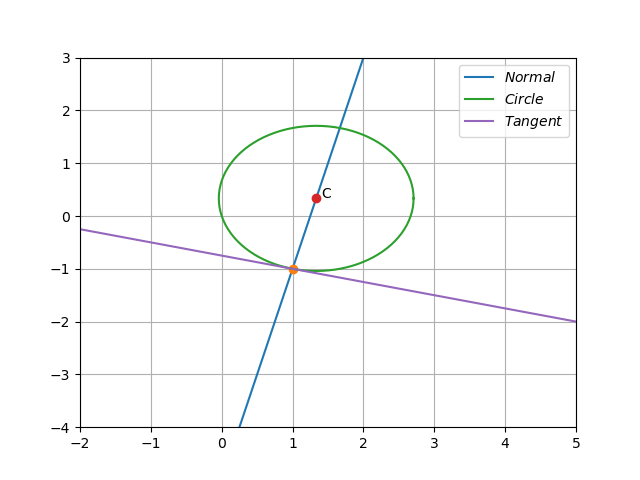
\includegraphics[width=\linewidth,height=\textheight,keepaspectratio]{Figure_1.png}

\end{figure}
\end{frame}
\end{document}